\documentclass{report}

\usepackage[T1]{fontenc}
\usepackage{graphicx}
\usepackage{pict2e}
\usepackage{xcolor}
\usepackage{amsmath}
\usepackage[rflt]{floatflt}
\usepackage{graphicx,subfigure,epic,eepic}
\usepackage[most]{tcolorbox}
\usepackage{float}
\usepackage{caption}
\usepackage{fullpage}
\usepackage{hyperref}
\usepackage{fancyhdr}
\pagestyle{fancy}
\lhead{}
\rhead{}
\cfoot{}
\usepackage[top=5mm,includehead,headheight=45pt,
             left=1.5cm,bottom=2cm,right=1.5cm,headsep=0.3cm]{geometry} 

%inkscapestuff
\usepackage{import}
\usepackage{pdfpages}
\usepackage{transparent}
\usepackage{xcolor}

\newcommand{\incfig}[2][1]{%
    \def\svgwidth{#1\columnwidth}
    \import{./figures/}{#2.pdf_tex}
}

\pdfsuppresswarningpagegroup=1





\title{{Summer Research Report} \\ {CSB, IISc}

\begin{figure}[H]\centering
	
\includegraphics[scale=0.05]{img/IIsc_logo.png}

\end{figure}

}
\author{Vaibhav Anand \\ 
BS MS student at IISER Pune, Batch of 26
\\

~\\
Under guidance of Mohit Kumar Jolly and Kishore Hari }

\begin{document}
\maketitle

\chapter*{May}
I started off with writing a function for asynchronus boolean update of a network based on ising formalism. Subsequently I used and understood how RACIPE works and understood the meaning of its equations. My goal was to explore as many directions/questions which might interest me as I could. 

I got interested in wether we have osscillations in the networks we consider and how dependent it is on the formalism and the boolean rules we use. 

I wanted to know how rare are osscillations and its dependence on the rules of the simulations since in most networks I looked at implementing ising formalism did not have many osscillatory steady states. 

I wanted to know how much of it is because of topology of the network and how much is it because of the rules of the simulations. 



I still haven't explored this direction to my satisfaction and would like to look into it in future. 


I compared the steady state distribution of GHL2 network obtained via RACIPE and ising formalism and calculated the JSD for the same. 

 


Briefly got interested in the question if certain RACIPE parameter ranges enrich for hybrid phenotypes and some enrich for terminal ( epithelial/mesenchymal ) phenotypes. 

The motivation was that there are parameter ranges for a simple toggle switch which do not allow for bistable solutions. I started wondering if there would be prameter similar parameter ranges in larger networks which allow for only certain phenotypes to occur. 

However, I did not up making much progress in this direction and moved on to boolean modelling from ODE modelling. And started reproducing data from papers. 

\chapter*{June }

\section{Read and analysed the following papers in depth}
 \begin{itemize}
 
 \item Robustness in phenotypic plasticity and heterogeneity patterns enabled by EMT networks

 \item Landscape of epithelial–mesenchymal plasticity as an emergent property of coordinated teams in regulatory networks

 
 \end{itemize}
Continued properly implementing code and reproduced some figures from the above mentioned papers.
\\
Then I proceeded to superficially look at some metrics I wanted to look at in may. 

\section{Two simulation based metrics}

\subsection{Time for convergencne }
The networks we considered tend to converge to a solution quite fast
I decided to look at the number of asynchronus updates taken (timesteps) to reach a steady state on average. 

Average time for convergence seems to be a function of number of edges and it saturates after a while. 
\begin{figure}[H]\centering 
	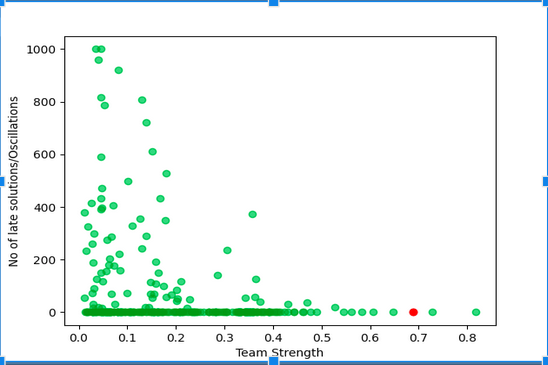
\includegraphics[scale=0.4]{img/time_for_covg_vs_teamstrength.png}
	\caption{Time for convergence vs Team strength}


\end{figure}
\subsubsection{Average time for covergence is lesser for hybrid states} 
Inputs which reached different basins were tracked and it was found that random inputs which evolved and reached hybrid states. It was found that the \textbf{ average } time for convergence was lesser for hybrid states than optimal (epithelial/mesenchymal) states. 

One possible reason could be that hybrid states have a smaller sized basin therefore inputs which fall into the hybrid basins are probably already quite hybrid or rather closer to the hybrid state state resulting in a small average. I'm yet to verify this. 

\subsection{Number of long range solutions (t>1000)/oscillations }
Teams structure tends to strictly restrict the number of long range solutions/osscillations at 0  
\begin{figure}[H]\centering 
	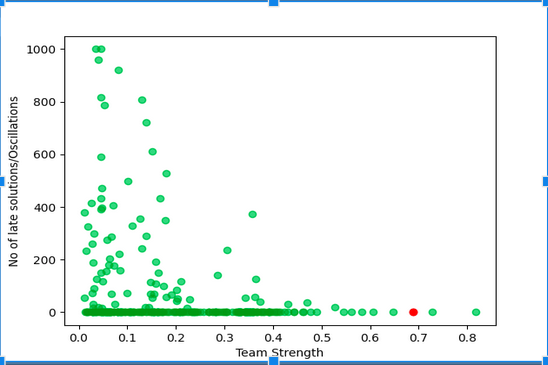
\includegraphics[scale=0.4]{img/time_for_covg_vs_teamstrength.png}
	\caption{Time for convergence vs Team strength}


\end{figure}

\section{Robustness Measures}
The robustness paper hadn't looked into robustness of EMT networks with respect to one node being consistently on.


Connectivity of small world network is robust to random node knockout. 
I also wanted to see if EMT networks topologies are robust to node knockout. 

For this I needed to figure out what topology based metric to look at. I started off with mean average path length but that did not give any significant results. I couldn't explore much in this direction but I would like to come back to this in future. 


\subsection{One node on}
It was found that EMT networks are robust to a node being on. 

\section{A static metric}

\section{Brief foray into }

\section{Unregulated Nodes}

\section{Three state formalism }


\section{Hybrid Islands}


\section{Consistently Unregulated nodes}





\end{document}

